\documentclass{article}
\usepackage{CJK}
\usepackage{amsmath}
\usepackage{amsthm}
\usepackage{amsfonts}
\usepackage{palatino}
\usepackage{xcolor}
\usepackage{geometry}
\usepackage{listings}
\usepackage{enumerate}
\usepackage[pdftex]{graphicx}
\geometry{left=2cm,right=2cm,top=3cm,bottom=3cm}
\pagestyle{myheadings}
\markright{Huiqian Yu/14300180118}
\setlength{\parindent}{0pt}
\newcommand{\ix}[1]{\intertext{{}#1}}
\newcommand{\dx}{\mathrm{d}\,x}
\newcommand{\dt}{\mathrm{d}\,t}
\newcommand{\dm}[1]{\mathrm{d}\,{}#1}
\newcommand{\ve}{\varepsilon}
\newcommand{\tp}{^\mathsf{T}}
\begin{document}

\definecolor{backcolour}{rgb}{0.95,0.95,0.92}
\begin{CJK*}{GBK}{song}
\begin{enumerate}
\item[1.2]
(a)
\begin{center}
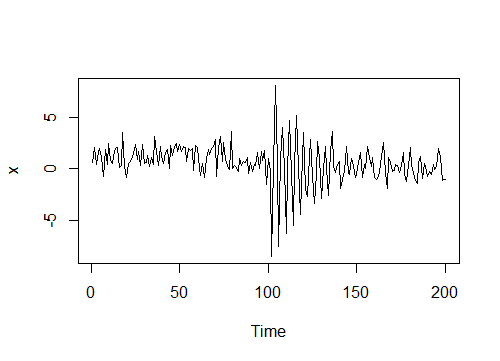
\includegraphics[width=8cm]{1.png}
\end{center}
(b)
\begin{center}
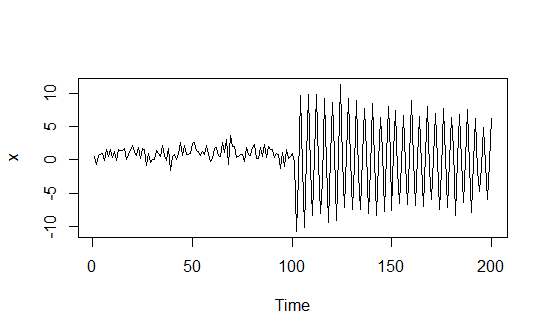
\includegraphics[width=8cm]{2.png}
\end{center}
(c)\\
The series (a) and (b) both changed violently after $t=100$, and become smooth over time.  
\begin{center}
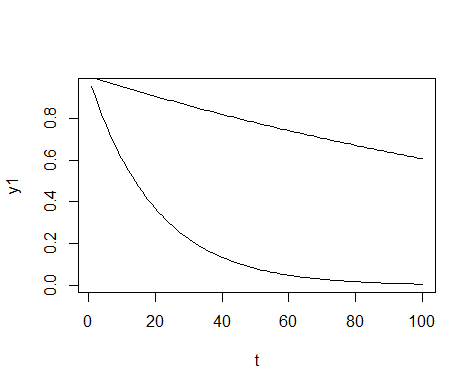
\includegraphics[width=8cm]{3.png}
\end{center}
From the plot of $e^{-t/20}$ and $e^{-t/200}$ above we can find that in the period of $t=100s$, $e^{-t/20}$ changed a lot, but $e^{-t/200}$ did not change much. That is in sympathy with we found from the plots in (a) and (b).\\
\item[1.5]
(a)\begin{align*}
\mu_{1x}(t)=s_t&=\left\{
                \begin{array}{ll}
                  0, & \hbox{$t=1,\cdots,100$;} \\
                  10e^{-(t-100)/20}\cos (2\pi t/4), & \hbox{$t=101,\cdots,200$.}
                \end{array}
              \right.\\
\mu_{2x}(t)=s_t&=\left\{
                \begin{array}{ll}
                  0, & \hbox{$t=1,\cdots,100$;} \\
                  10e^{-(t-100)/200}\cos (2\pi t/4), & \hbox{$t=101,\cdots,200$.}
                \end{array}
              \right.
\end{align*}
\begin{center}
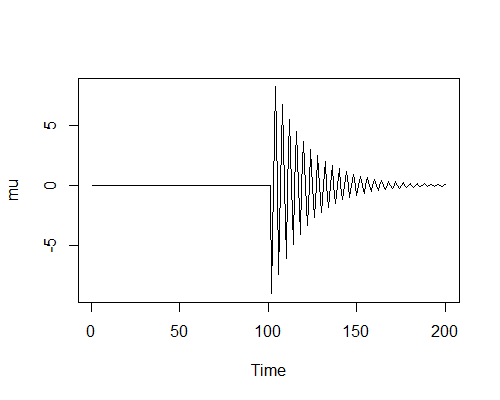
\includegraphics[width=8cm]{4.png}
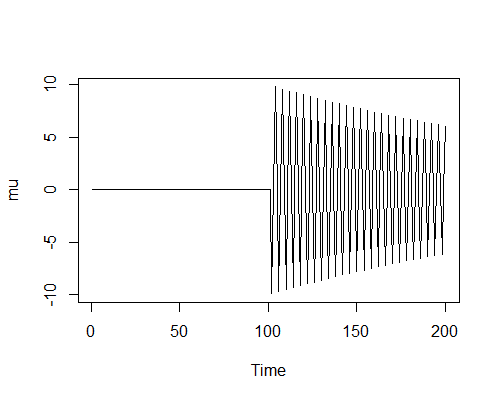
\includegraphics[width=8cm]{5.png}
\end{center}
(b)
\begin{align*}
\gamma_x(s,t)&=\mathbb{E}(X_s-\mu_s)(X_t-\mu_t)\\
&=\mathbb{E}w_sw_t\\
&=0
\end{align*}

\item[1.8]

(a)
\begin{align*}
\ix{Assume that $x_{t-1}=\delta {t-1}+\sum\limits_{k=1}^{t-1} w_k$, then}
     x_t&= \delta+x_{t-1}+w_t\\
        &= \delta t+ \sum\limits_{k=1}^{t} w_k\\
\ix{Since} x_1&=\delta+0+w_1
\end{align*}
By mathematical induction, the model can be written as $x_t= \delta t+ \sum\limits_{k=1}^{t} w_k$
(b)\\
\begin{align*}
\mu_xt&=\delta t\\
\gamma_x(s,t)&=\mathbb{E}\sum\limits_{k\le t} w_k \sum\limits_{j\le s} w_j\\
&=\min(s,t)\sigma^2
\end{align*}
(c)\\
From the calculation in (b), $\gamma(s,t)$ not only depends on $|s-t|$, so $x_t$ is not stationary.\\
(d)\\

\begin{align*}
\rho_x(t-1,t)&=\dfrac{\gamma(t-1,t)}{\sqrt{\gamma(t-1,t-1)\gamma(t,t)}}\\
&=\dfrac{(t-1)\sigma^2}{\sqrt{(t-1)t\sigma^4}}\\
&=\sqrt{\dfrac{t-1}{t}}
\end{align*}
It implicates that as $t\rightarrow\infty$, $x_t$ is nearly proportional to $x_{t-1}$.\\
(e)\\
\begin{align*}
\ix{Let}y_t&= x_t-x_{t-1}\\
\ix{Then}y_t&=\delta + w_t-w_{t-1}\\
w_t-w_{t-1}&\sim (0,2\sigma_w^2)\\
\ix{So}\mu_yt&=\delta\\
\gamma_y(s,t)&=\left\{
                 \begin{array}{ll}
                   0, & \hbox{$|s-t|>1$;} \\
                   -2\sigma_w^2, & \hbox{$|s-t|=1$.}
                 \end{array}
               \right.
\end{align*}
\item[1.14]
\begin{align*}
\ix{(a)}    \mathbb{E}(y_t)&= \mathbb{E}e^{x_t}\\
        &=e^{\mu_x+\dfrac{1}{2}\gamma(0)}\\
\ix{(b)}     \gamma_y(s,t)&= \mathbb{E}(e^{x_t}-\mu_y)(e^{x_s}-\mu_y)\\
        &=\mathbb{E}(e^{x_t+x_s}-2\mu_y(e^{x_s}+e^{x_t})+\mu_y^2)\\
        &=e^{\mu_x+\gamma(0)}-3e^{2\mu_x+\gamma(0)}
\end{align*}

\item[1.18]

\begin{align*}
\ix{Since $\sum |\phi_j|$ is converge, when $j$ is big enough,}
    |\phi_j|&<1,\\
\ix{so,} |\phi_j||phi_{j+h}|&<\max(|\phi_j|,\|\phi_{j+h}|)^2<1,\\
\ix{thus,} \gamma(h)&=\sigma_w^2\sum |\phi_j||phi_{j+h}|
\end{align*}
is converge.

\item[1.25]
\begin{align*}
    \ix{We directly prove (b), for any vector $\mathbf{y}$}
        &mathbf{y}\tp\mathbb{E}\left[(X-\mathbb{E}X)(X-\mathbb{E}X)\tp\right]mathbf{y}\\
    &=\mathbb{E}\left[mathbf{y}\tp(X-\mathbb{E}X)\right]^2\\
&\ge 0
\end{align*}
Thus, the sample autocovariance is a non-negative definite function.


\end{enumerate}
\end{CJK*}
\end{document}
